\section{Le Projet}
\subsection{Objet du document}

Ce document a pour objectif le suivi du projet "Atelier logiciel - système de transmission"
Vous trouverez dans ce document l'ensemble des itérations, les tests réalisés, et les modifications apportées tout au long du projet.

\subsection{Cahier des charges}

L'objectif consiste à transmettre un message d'un point d'entrée à un point de sortie, via un canal de transmission (ou de communication). Le message d'entrée est émis par une source d'entrée. Les messages considérés dans ce projet seront des suites de symboles binaires (0 ou 1) correspondant à des informations échantillonnées et quantifiées sur deux niveaux logiques. Le message de sortie sera - autant que faire se peut - semblable au message d'entrée. Ce dernier étant incapable de traverser le canal de propagation tel quel, on l'adaptera aux caractéristiques physiques du canal en le convertissant au moyen d'un transducteur en un " vecteur " adapté à la transmission, appelé signal.

Ce dernier sera injecté dans le canal au moyen d'un émetteur. À l'autre extrémité du canal, il sera récupéré et traité par le récepteur et le transducteur de réception.

Les principaux canaux de transmission rencontrés dans la nature sont : le canal Hertzien (espace libre), le canal guidé électrique (câble), le canal guidé Optique (fibre), le canal acoustique aérien et le canal acoustique sous-marin. Chaque canal de propagation devant être utilisé à une fréquence bien particulière, le message est transposé autour de cette fréquence par l'opération de modulation. En outre, le canal sera une source de bruit pour les signaux qu'il transporte. Les principales sources de bruit rencontrées en pratique sont : la dispersion de trajets, la dispersion chromatique, le bruit de détection (grenaille), le bruit thermique et le bruit d'amplification.

Par la suite, chaque composant du système de transmission entre la source et la destination sera dénommé transmetteur.

\begin{figure}[H]
    \centering
    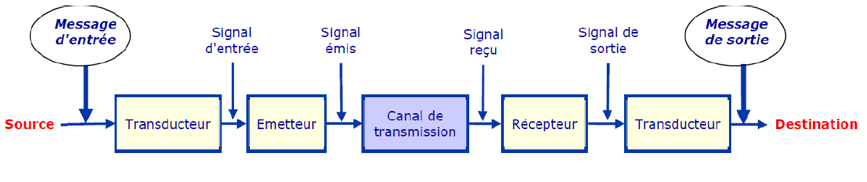
\includegraphics[width=1\textwidth]{image 1.png}
    \caption{\label{fig:image1}Composants de la chaine de transmission.}
\end{figure}

\pagebreak

\section{Iteration n°1}
\subsection{Objectifs}

L'objectif de cette première itération est avant tout de prendre en main la chaine de transmission.

Pour cette itération, la chaine respectera les propriétés suivantes :

La source émet une séquence booléenne soit fixée, soit aléatoire.
Le transmetteur logique parfait se contente, à la réception d'un signal, de l'émettre tel quel vers les destinations qui lui sont connectées.
La destination se contente de recevoir le signal du composant sur lequel elle est connectée.
Des sondes logiques permettent de visualiser les signaux émis par la source et le transmetteur parfait.
L'application principale calcule le taux d'erreur binaire (TEB) du système.

Voici un schéma de la chaine :

\begin{figure}[H]
    \centering
    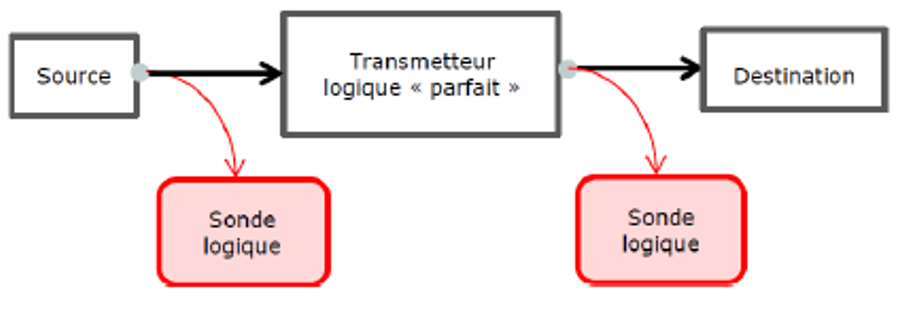
\includegraphics[width=1\textwidth]{image 2.png}
    \caption{\label{fig:image2}Chaine de transmission itération 1.}
\end{figure}

\subsection{Choix d'implémentation}

Pour permettre une utilisation simple et rapide du simulateur, la mise en place de scripts de compilation, de création de documentation et d'éxécution
ont été mis en place. Ces scripts sont disponibles à la racine du projet.
Il est donc possible de compiler puis tester le simulateur en utilisant les divers arguments spécifiés dans le readme.

Les différentes fonctionnalitées implémentées dans l'étape 1 (transmetteur parfait) sont les suivantes:
nbsample

En prévision d'une potentielle fusion de binômes, nous avons décidé de mettre en place une architecture logicielle versionné sur git.
Elle nous permettra à chacun de reprendre le projet et de travailler sur des fonctionnalitées différentes sans avoir à se soucier des conflits de version.

\subsection{Actions réalisées}

\subsubsection{Sources}

Dans un premier temps, nous avons créé deux classes sources. Une source fixe, qui envoie toujours la même séquence de données. Puis une source aléatoire qui envoie une nouvelle séquence à chaque appel.

\subsubsection{Transmetteur}

Par la suite, nous avons créé un transmetteur parfait. Il joue le rôle du canal de propagation. Pour ce transmetteur parfait, le canal transmet exactement ce qu'il reçoit.

\subsubsection{Destination}

Enfin, nous avons créé une destination. Cette classe joue le rôle de récepteur dans la chaine de transmission.

\subsection{Simulation}

Lors de l'execution de la commande: 

\begin{figure}[H]
    \centering
    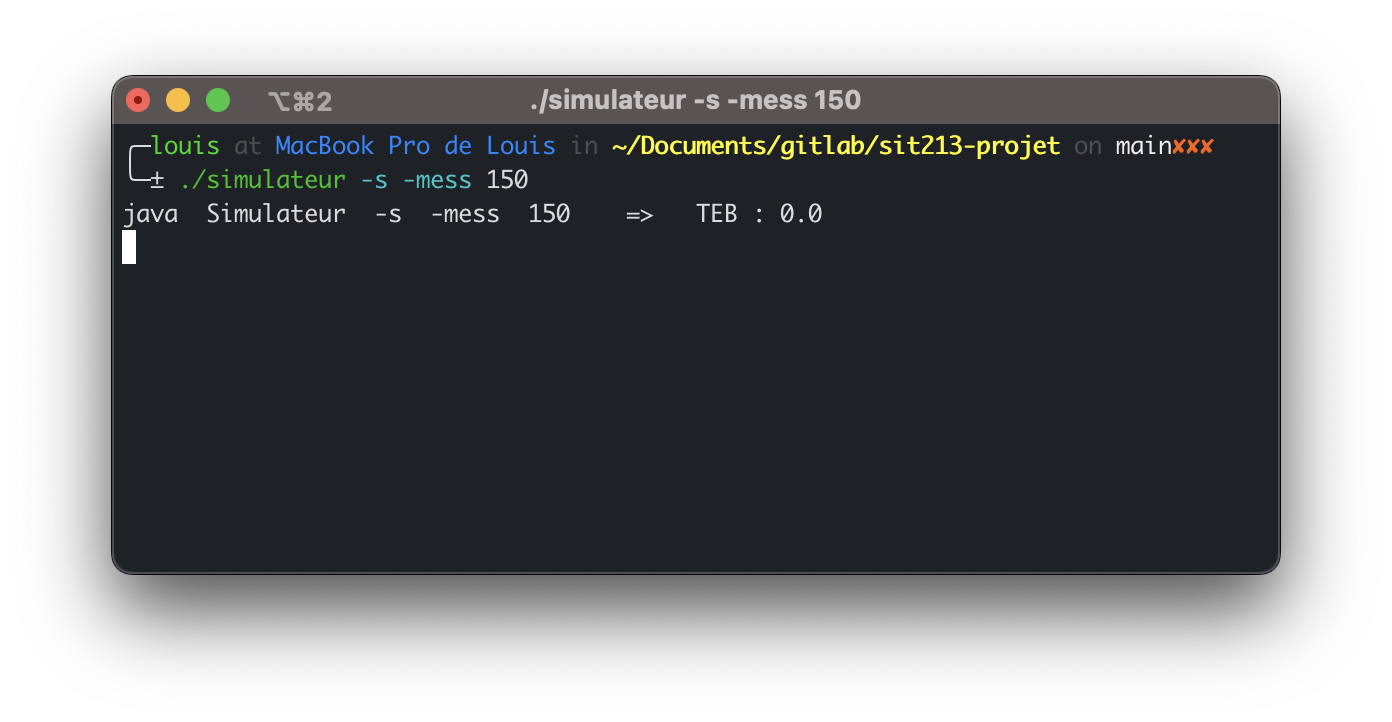
\includegraphics[width=\textwidth]{term_1.png}
    \caption{terminal}
\end{figure}

On constate lors de l'execution du script l'affichacge d'un signal identique sur la source et la destination (voir figure 2). Cela coincide 
avec le fait que le transmetteur est parfait et que le signal n'est donc pas modifié lors de la transmission vers la destination.
Le TEB est égal à 0 comme attendu.

\begin{figure}[H]
    \centering
    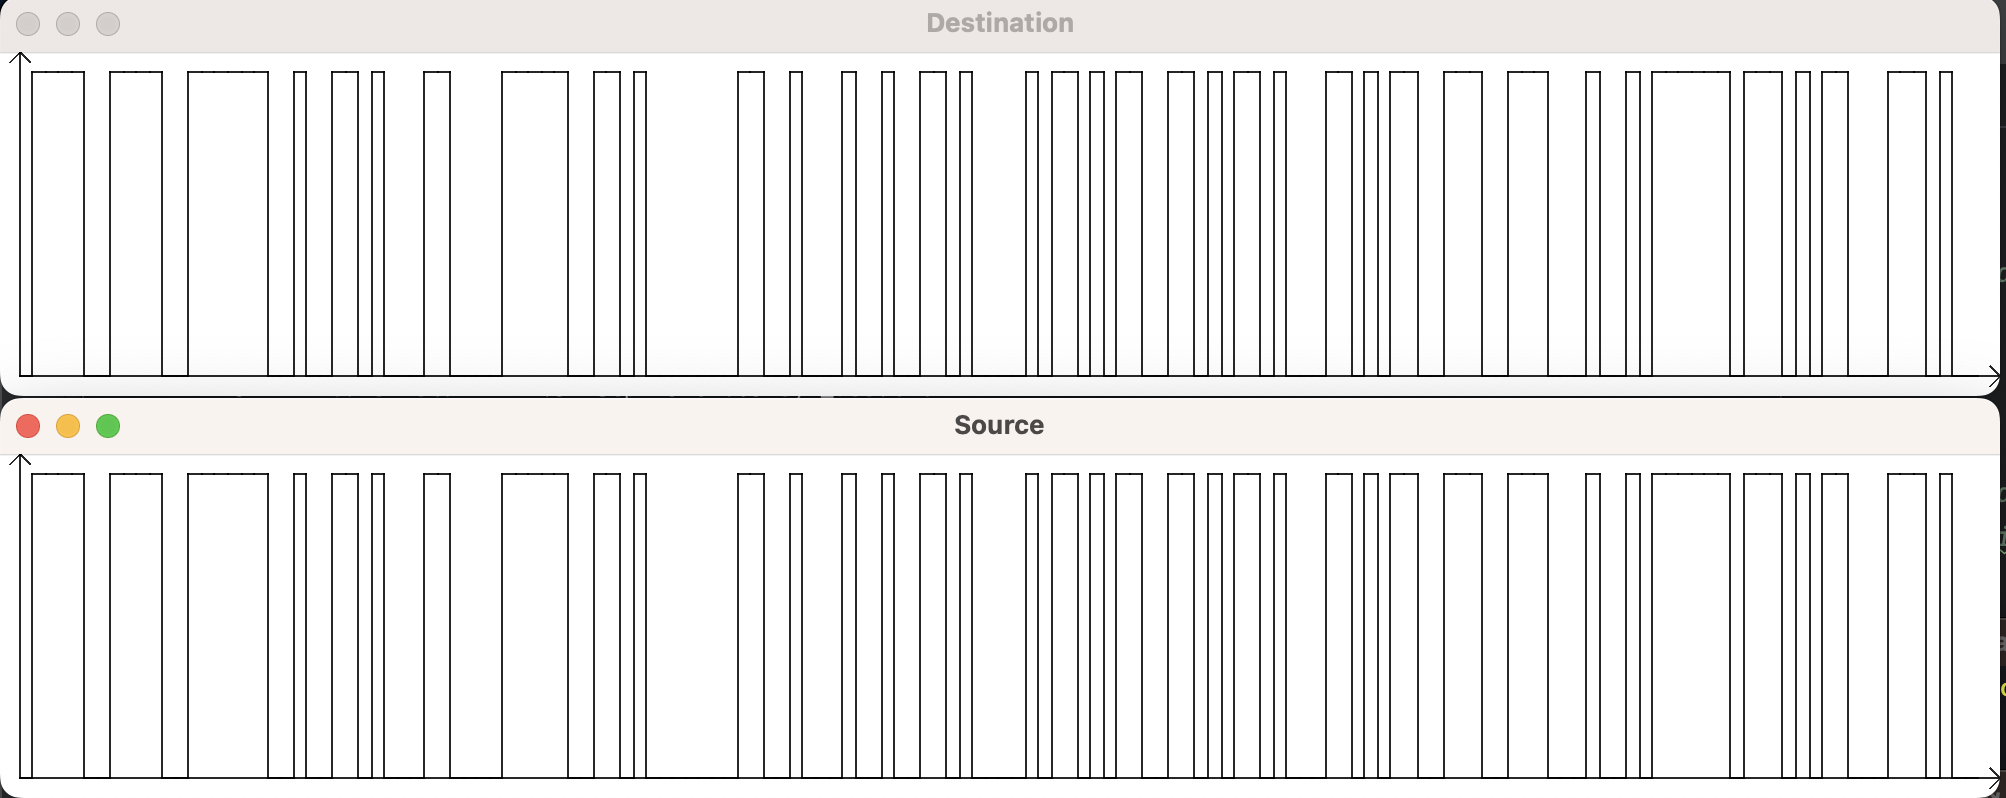
\includegraphics[width=\textwidth]{s_r_100.png}
    \caption{Execution du programme}
\end{figure}

\pagebreak

Executer le programme deux fois en utilisant la meme graine nous permet d'obtenir la meme génération de signal.
Cela nous sera utile dans le cadre de tests ultérieurs afin de s'assurer du bon fonctionnement du simulateur dans plusieurs situations différentes.

\begin{figure}[H]
    \centering
    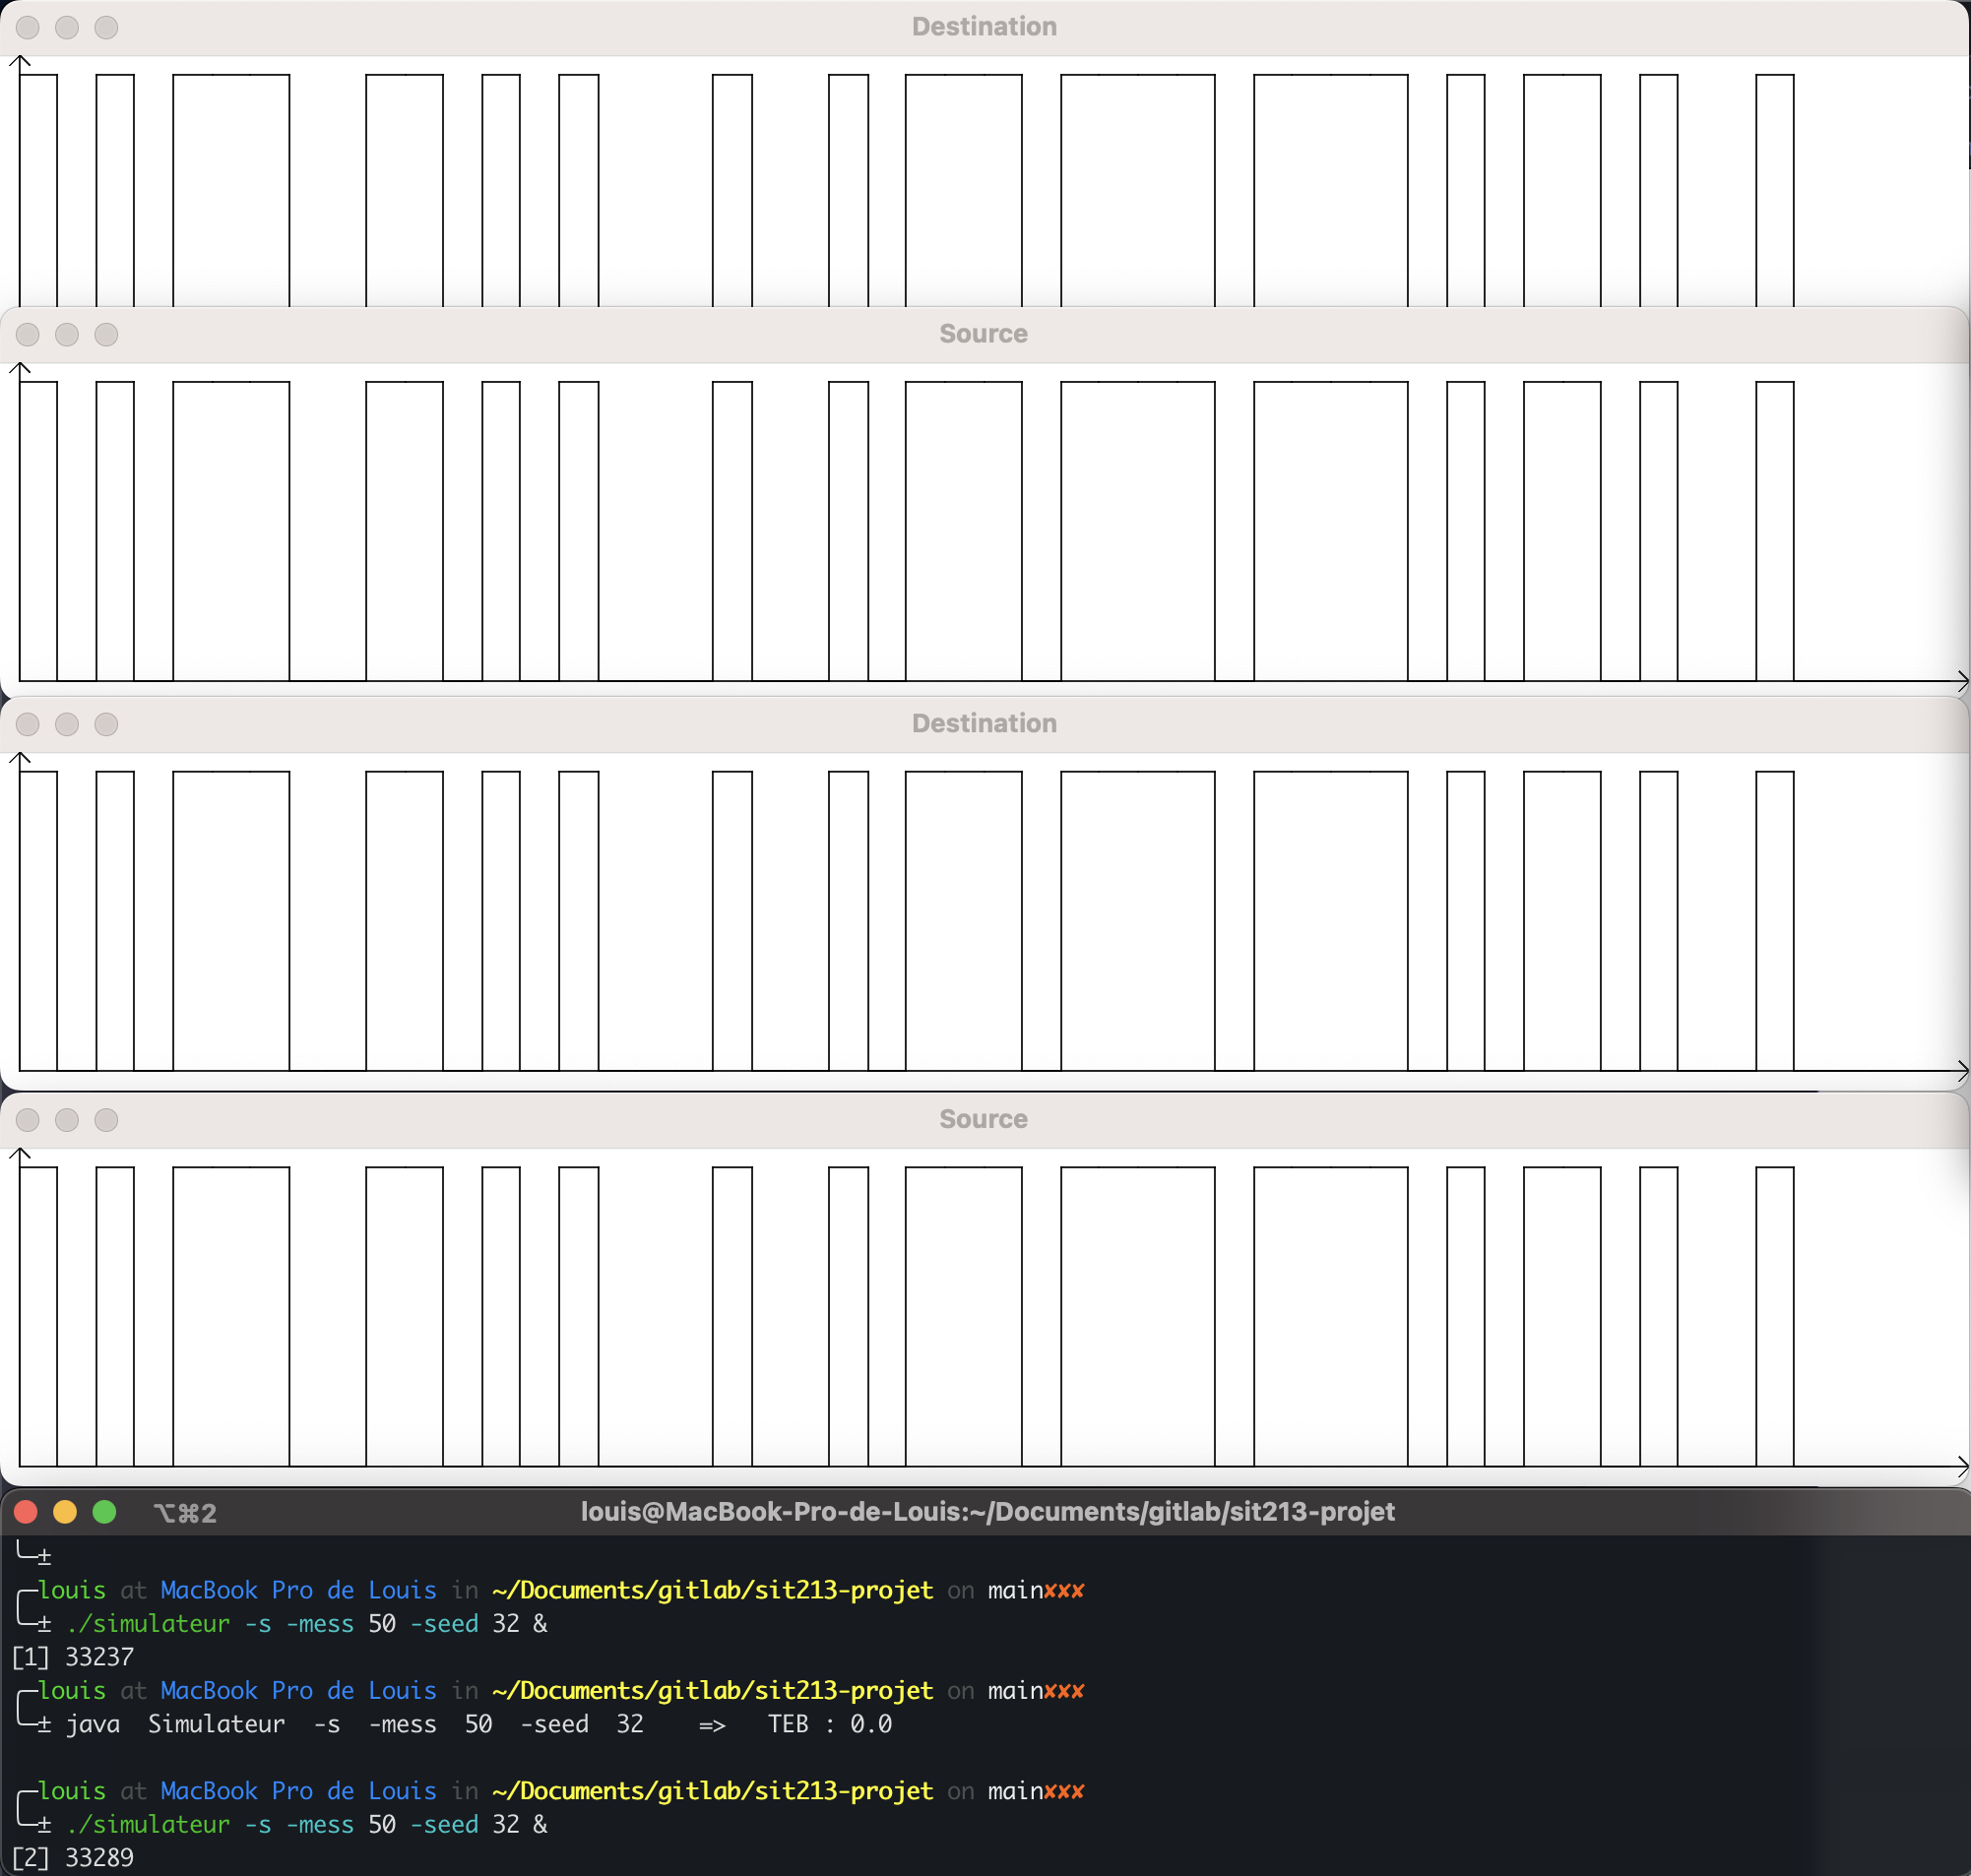
\includegraphics[width=\textwidth]{s_r_50.png}
    \caption{Exemple utilisation d'une "seed"}
\end{figure}

Nous observons que la sortie du transmetteur est purement identique à la source. C'est normal car il s'agit d'un canal parfait. Le TEB est donc de 0.

\subsection{Conclusion}

Cette première étape a été très utile dans la compréhension de l'architecture logicielle mise à disposition.
Cela aura été l'occasion de commencer à penser à l'organisation du travail d'équipe à venir et de mettre en place des outils de travail collaboratif.
Par ailleurs, notre chaine de transmission est fonctionnelle, nous sommes en mesure de choisir le type de source et observer la sortie du canal.
Pour le moment, nous n'avons qu'un seul type de transmetteur et que deux types de sources. Par la suite, nous serons amenés à mettre en œuvre une chaine de transmission avec des signaux analogiques et des canaux de propagations non-parfaits.